% Options for packages loaded elsewhere
\PassOptionsToPackage{unicode}{hyperref}
\PassOptionsToPackage{hyphens}{url}
\PassOptionsToPackage{dvipsnames,svgnames,x11names}{xcolor}
%
\documentclass[
  letterpaper,
  DIV=11,
  numbers=noendperiod]{scrartcl}

\usepackage{amsmath,amssymb}
\usepackage{iftex}
\ifPDFTeX
  \usepackage[T1]{fontenc}
  \usepackage[utf8]{inputenc}
  \usepackage{textcomp} % provide euro and other symbols
\else % if luatex or xetex
  \usepackage{unicode-math}
  \defaultfontfeatures{Scale=MatchLowercase}
  \defaultfontfeatures[\rmfamily]{Ligatures=TeX,Scale=1}
\fi
\usepackage{lmodern}
\ifPDFTeX\else  
    % xetex/luatex font selection
\fi
% Use upquote if available, for straight quotes in verbatim environments
\IfFileExists{upquote.sty}{\usepackage{upquote}}{}
\IfFileExists{microtype.sty}{% use microtype if available
  \usepackage[]{microtype}
  \UseMicrotypeSet[protrusion]{basicmath} % disable protrusion for tt fonts
}{}
\makeatletter
\@ifundefined{KOMAClassName}{% if non-KOMA class
  \IfFileExists{parskip.sty}{%
    \usepackage{parskip}
  }{% else
    \setlength{\parindent}{0pt}
    \setlength{\parskip}{6pt plus 2pt minus 1pt}}
}{% if KOMA class
  \KOMAoptions{parskip=half}}
\makeatother
\usepackage{xcolor}
\usepackage[top=1in, bottom=1in, left=1in, right=1in]{geometry}
\setlength{\emergencystretch}{3em} % prevent overfull lines
\setcounter{secnumdepth}{-\maxdimen} % remove section numbering
% Make \paragraph and \subparagraph free-standing
\makeatletter
\ifx\paragraph\undefined\else
  \let\oldparagraph\paragraph
  \renewcommand{\paragraph}{
    \@ifstar
      \xxxParagraphStar
      \xxxParagraphNoStar
  }
  \newcommand{\xxxParagraphStar}[1]{\oldparagraph*{#1}\mbox{}}
  \newcommand{\xxxParagraphNoStar}[1]{\oldparagraph{#1}\mbox{}}
\fi
\ifx\subparagraph\undefined\else
  \let\oldsubparagraph\subparagraph
  \renewcommand{\subparagraph}{
    \@ifstar
      \xxxSubParagraphStar
      \xxxSubParagraphNoStar
  }
  \newcommand{\xxxSubParagraphStar}[1]{\oldsubparagraph*{#1}\mbox{}}
  \newcommand{\xxxSubParagraphNoStar}[1]{\oldsubparagraph{#1}\mbox{}}
\fi
\makeatother


\providecommand{\tightlist}{%
  \setlength{\itemsep}{0pt}\setlength{\parskip}{0pt}}\usepackage{longtable,booktabs,array}
\usepackage{calc} % for calculating minipage widths
% Correct order of tables after \paragraph or \subparagraph
\usepackage{etoolbox}
\makeatletter
\patchcmd\longtable{\par}{\if@noskipsec\mbox{}\fi\par}{}{}
\makeatother
% Allow footnotes in longtable head/foot
\IfFileExists{footnotehyper.sty}{\usepackage{footnotehyper}}{\usepackage{footnote}}
\makesavenoteenv{longtable}
\usepackage{graphicx}
\makeatletter
\def\maxwidth{\ifdim\Gin@nat@width>\linewidth\linewidth\else\Gin@nat@width\fi}
\def\maxheight{\ifdim\Gin@nat@height>\textheight\textheight\else\Gin@nat@height\fi}
\makeatother
% Scale images if necessary, so that they will not overflow the page
% margins by default, and it is still possible to overwrite the defaults
% using explicit options in \includegraphics[width, height, ...]{}
\setkeys{Gin}{width=\maxwidth,height=\maxheight,keepaspectratio}
% Set default figure placement to htbp
\makeatletter
\def\fps@figure{htbp}
\makeatother

\KOMAoption{captions}{tableheading}
\makeatletter
\@ifpackageloaded{caption}{}{\usepackage{caption}}
\AtBeginDocument{%
\ifdefined\contentsname
  \renewcommand*\contentsname{Table of contents}
\else
  \newcommand\contentsname{Table of contents}
\fi
\ifdefined\listfigurename
  \renewcommand*\listfigurename{List of Figures}
\else
  \newcommand\listfigurename{List of Figures}
\fi
\ifdefined\listtablename
  \renewcommand*\listtablename{List of Tables}
\else
  \newcommand\listtablename{List of Tables}
\fi
\ifdefined\figurename
  \renewcommand*\figurename{Figure}
\else
  \newcommand\figurename{Figure}
\fi
\ifdefined\tablename
  \renewcommand*\tablename{Table}
\else
  \newcommand\tablename{Table}
\fi
}
\@ifpackageloaded{float}{}{\usepackage{float}}
\floatstyle{ruled}
\@ifundefined{c@chapter}{\newfloat{codelisting}{h}{lop}}{\newfloat{codelisting}{h}{lop}[chapter]}
\floatname{codelisting}{Listing}
\newcommand*\listoflistings{\listof{codelisting}{List of Listings}}
\makeatother
\makeatletter
\makeatother
\makeatletter
\@ifpackageloaded{caption}{}{\usepackage{caption}}
\@ifpackageloaded{subcaption}{}{\usepackage{subcaption}}
\makeatother

\ifLuaTeX
  \usepackage{selnolig}  % disable illegal ligatures
\fi
\usepackage{bookmark}

\IfFileExists{xurl.sty}{\usepackage{xurl}}{} % add URL line breaks if available
\urlstyle{same} % disable monospaced font for URLs
\hypersetup{
  pdftitle={home\_work\_test},
  pdfauthor={Baodong Zhang},
  colorlinks=true,
  linkcolor={blue},
  filecolor={Maroon},
  citecolor={Blue},
  urlcolor={Blue},
  pdfcreator={LaTeX via pandoc}}


\title{home\_work\_test}
\author{Baodong Zhang}
\date{}

\begin{document}
\maketitle


\subsection{Introduction}\label{introduction}

Cardiovascular diseases (CVD) are a leading cause of mortality
worldwide. This report investigates whether cardiovascular disease
(variable `cardio`) can be explained by other variables such as age,
gender, blood pressure, BMI, and lifestyle factors like smoking, alcohol
consumption, and physical activity. The analysis is based on a dataset
containing various health metrics.

\newpage

\subsection{Chapter 01 Data
Preparation}\label{chapter-01-data-preparation}

Task 1: Transform the variables of the data set to appropriate data
types and assign factor labels for the categorical variables.

\begin{table}[!h]
\centering
\caption{Data Overview}
\centering
\begin{tabular}[t]{l|l|l|r|l}
\hline
\cellcolor[HTML]{D3D3D3}{\textbf{ }} & \cellcolor[HTML]{D3D3D3}{\textbf{variable}} & \cellcolor[HTML]{D3D3D3}{\textbf{class}} & \cellcolor[HTML]{D3D3D3}{\textbf{unique\_values}} & \cellcolor[HTML]{D3D3D3}{\textbf{example\_values}}\\
\hline
\cellcolor{gray!10}{id} & \cellcolor{gray!10}{id} & \cellcolor{gray!10}{integer} & \cellcolor{gray!10}{5000} & \cellcolor{gray!10}{24628, 66016, 36566, 30609, 53555}\\
\hline
age & age & numeric & 1753 & 58.68, 55.89, 60.11, 47.87, 52.16\\
\hline
\cellcolor{gray!10}{gender} & \cellcolor{gray!10}{gender} & \cellcolor{gray!10}{factor} & \cellcolor{gray!10}{2} & \cellcolor{gray!10}{Male, Female}\\
\hline
height & height & integer & 61 & 159, 167, 169, 163, 165\\
\hline
\cellcolor{gray!10}{weight} & \cellcolor{gray!10}{weight} & \cellcolor{gray!10}{numeric} & \cellcolor{gray!10}{115} & \cellcolor{gray!10}{59, 89, 78, 75, 73}\\
\hline
ap\_hi & ap\_hi & integer & 65 & 120, 140, 12, 110, 150\\
\hline
\cellcolor{gray!10}{ap\_lo} & \cellcolor{gray!10}{ap\_lo} & \cellcolor{gray!10}{integer} & \cellcolor{gray!10}{54} & \cellcolor{gray!10}{80, 90, 79, 70, 69}\\
\hline
cholesterol & cholesterol & factor & 3 & normal, above normal, well above normal\\
\hline
\cellcolor{gray!10}{gluc} & \cellcolor{gray!10}{gluc} & \cellcolor{gray!10}{factor} & \cellcolor{gray!10}{3} & \cellcolor{gray!10}{normal, above normal, well above normal}\\
\hline
smoke & smoke & factor & 2 & no, yes\\
\hline
\cellcolor{gray!10}{alco} & \cellcolor{gray!10}{alco} & \cellcolor{gray!10}{factor} & \cellcolor{gray!10}{2} & \cellcolor{gray!10}{no, yes}\\
\hline
active & active & factor & 2 & yes, no\\
\hline
\cellcolor{gray!10}{cardio} & \cellcolor{gray!10}{cardio} & \cellcolor{gray!10}{factor} & \cellcolor{gray!10}{2} & \cellcolor{gray!10}{absent, present}\\
\hline
\end{tabular}
\end{table}

\newpage

\subsection{Chapter 2: Outlier
Detection}\label{chapter-2-outlier-detection}

Task 2: Check the continuous variables for outliers and remove
implausible values.

\begin{table}[!h]
\centering
\caption{Summary of Continuous Variables}
\centering
\begin{tabular}[t]{l|l|l|l|l|l}
\hline
\cellcolor[HTML]{D3D3D3}{\textbf{ }} & \cellcolor[HTML]{D3D3D3}{\textbf{     age}} & \cellcolor[HTML]{D3D3D3}{\textbf{    height}} & \cellcolor[HTML]{D3D3D3}{\textbf{    weight}} & \cellcolor[HTML]{D3D3D3}{\textbf{    ap\_hi}} & \cellcolor[HTML]{D3D3D3}{\textbf{    ap\_lo}}\\
\hline
\cellcolor{gray!10}{} & \cellcolor{gray!10}{Min.   :39.16} & \cellcolor{gray!10}{Min.   : 60.0} & \cellcolor{gray!10}{Min.   : 21.00} & \cellcolor{gray!10}{Min.   :  10.0} & \cellcolor{gray!10}{Min.   :  40.0}\\
\hline
 & 1st Qu.:48.20 & 1st Qu.:159.0 & 1st Qu.: 64.00 & 1st Qu.: 120.0 & 1st Qu.:  80.0\\
\hline
\cellcolor{gray!10}{} & \cellcolor{gray!10}{Median :53.98} & \cellcolor{gray!10}{Median :165.0} & \cellcolor{gray!10}{Median : 72.00} & \cellcolor{gray!10}{Median : 120.0} & \cellcolor{gray!10}{Median :  80.0}\\
\hline
 & Mean   :53.31 & Mean   :164.3 & Mean   : 74.01 & Mean   : 126.7 & Mean   :  96.1\\
\hline
\cellcolor{gray!10}{} & \cellcolor{gray!10}{3rd Qu.:58.48} & \cellcolor{gray!10}{3rd Qu.:170.0} & \cellcolor{gray!10}{3rd Qu.: 82.00} & \cellcolor{gray!10}{3rd Qu.: 140.0} & \cellcolor{gray!10}{3rd Qu.:  90.0}\\
\hline
 & Max.   :64.90 & Max.   :200.0 & Max.   :180.00 & Max.   :1420.0 & Max.   :8099.0\\
\hline
\end{tabular}
\end{table}

\textbf{Boxplot before outliers are removed}:

\begin{center}
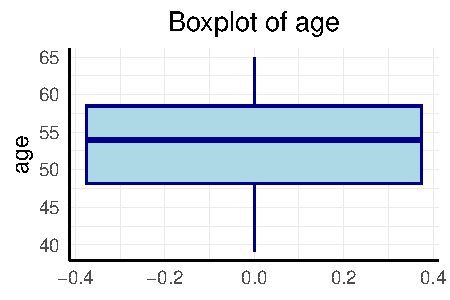
\includegraphics{home_work_test_files/figure-pdf/unnamed-chunk-3-1.pdf}
\end{center}

\begin{center}
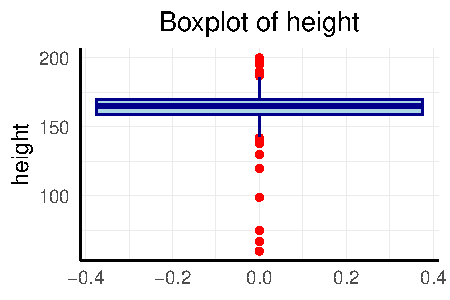
\includegraphics{home_work_test_files/figure-pdf/unnamed-chunk-3-2.pdf}
\end{center}

\begin{center}
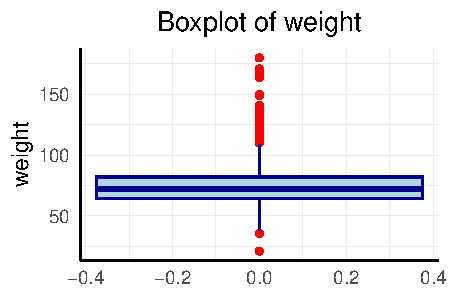
\includegraphics{home_work_test_files/figure-pdf/unnamed-chunk-3-3.pdf}
\end{center}

\begin{center}
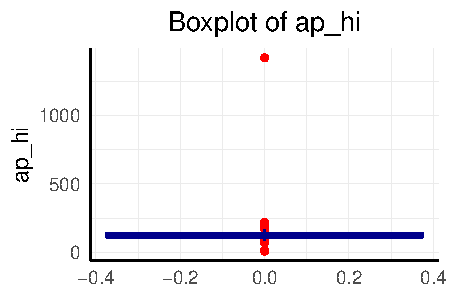
\includegraphics{home_work_test_files/figure-pdf/unnamed-chunk-3-4.pdf}
\end{center}

\begin{center}
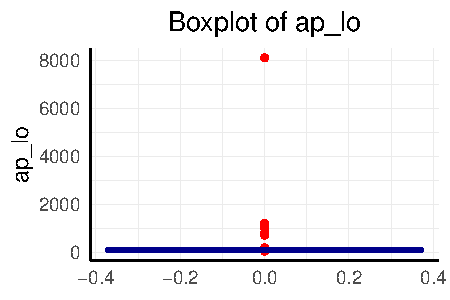
\includegraphics{home_work_test_files/figure-pdf/unnamed-chunk-3-5.pdf}
\end{center}

\newpage

\begin{table}[!h]
\centering
\caption{Summary of Continuous Variables (outliers are removed)}
\centering
\begin{tabular}[t]{l|l|l|l|l|l}
\hline
\cellcolor[HTML]{D3D3D3}{\textbf{ }} & \cellcolor[HTML]{D3D3D3}{\textbf{     age}} & \cellcolor[HTML]{D3D3D3}{\textbf{    height}} & \cellcolor[HTML]{D3D3D3}{\textbf{    weight}} & \cellcolor[HTML]{D3D3D3}{\textbf{    ap\_hi}} & \cellcolor[HTML]{D3D3D3}{\textbf{    ap\_lo}}\\
\hline
\cellcolor{gray!10}{} & \cellcolor{gray!10}{Min.   :39.16} & \cellcolor{gray!10}{Min.   :130.0} & \cellcolor{gray!10}{Min.   : 40.00} & \cellcolor{gray!10}{Min.   : 70.0} & \cellcolor{gray!10}{Min.   : 53.00}\\
\hline
 & 1st Qu.:48.19 & 1st Qu.:159.0 & 1st Qu.: 64.00 & 1st Qu.:120.0 & 1st Qu.: 80.00\\
\hline
\cellcolor{gray!10}{} & \cellcolor{gray!10}{Median :53.97} & \cellcolor{gray!10}{Median :165.0} & \cellcolor{gray!10}{Median : 71.00} & \cellcolor{gray!10}{Median :120.0} & \cellcolor{gray!10}{Median : 80.00}\\
\hline
 & Mean   :53.30 & Mean   :164.4 & Mean   : 73.71 & Mean   :126.4 & Mean   : 81.25\\
\hline
\cellcolor{gray!10}{} & \cellcolor{gray!10}{3rd Qu.:58.44} & \cellcolor{gray!10}{3rd Qu.:170.0} & \cellcolor{gray!10}{3rd Qu.: 82.00} & \cellcolor{gray!10}{3rd Qu.:140.0} & \cellcolor{gray!10}{3rd Qu.: 90.00}\\
\hline
 & Max.   :64.90 & Max.   :197.0 & Max.   :136.00 & Max.   :200.0 & Max.   :120.00\\
\hline
\end{tabular}
\end{table}

\textbf{Boxplot after outliers are removed:}

\begin{center}
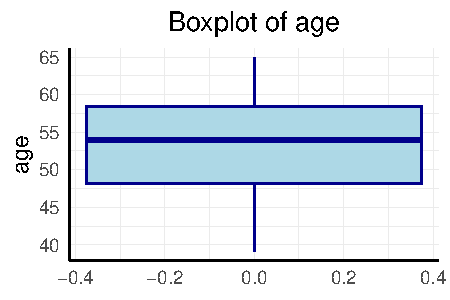
\includegraphics{home_work_test_files/figure-pdf/unnamed-chunk-6-1.pdf}
\end{center}

\begin{center}
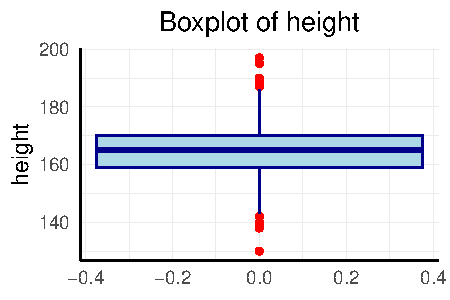
\includegraphics{home_work_test_files/figure-pdf/unnamed-chunk-6-2.pdf}
\end{center}

\begin{center}
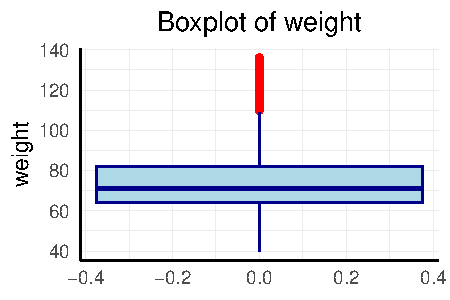
\includegraphics{home_work_test_files/figure-pdf/unnamed-chunk-6-3.pdf}
\end{center}

\begin{center}
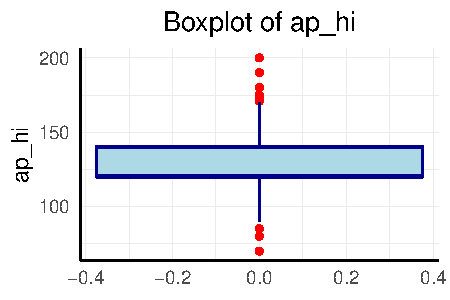
\includegraphics{home_work_test_files/figure-pdf/unnamed-chunk-6-4.pdf}
\end{center}

\begin{center}
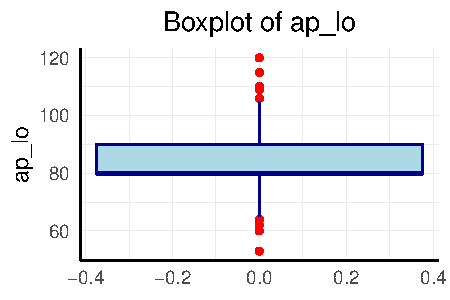
\includegraphics{home_work_test_files/figure-pdf/unnamed-chunk-6-5.pdf}
\end{center}

\newpage

\subsection{Chapter 3: BMI Calculation}\label{chapter-3-bmi-calculation}

Task 3: Create a new variable BMI and provide a summary table for the
variable BMI for both cardio groups.

\begin{table}[!h]
\centering
\caption{Summary table for BMI grouped by cardio}
\centering
\begin{tabular}[t]{l|r|r|r|r|r|r}
\hline
\cellcolor[HTML]{D3D3D3}{\textbf{cardio}} & \cellcolor[HTML]{D3D3D3}{\textbf{count}} & \cellcolor[HTML]{D3D3D3}{\textbf{mean\_BMI}} & \cellcolor[HTML]{D3D3D3}{\textbf{median\_BMI}} & \cellcolor[HTML]{D3D3D3}{\textbf{sd\_BMI}} & \cellcolor[HTML]{D3D3D3}{\textbf{min\_BMI}} & \cellcolor[HTML]{D3D3D3}{\textbf{max\_BMI}}\\
\hline
\cellcolor{gray!10}{absent} & \cellcolor{gray!10}{2495} & \cellcolor{gray!10}{26.34} & \cellcolor{gray!10}{25.34} & \cellcolor{gray!10}{4.62} & \cellcolor{gray!10}{15.82} & \cellcolor{gray!10}{50.41}\\
\hline
present & 2384 & 28.31 & 27.18 & 5.23 & 16.71 & 54.36\\
\hline
\end{tabular}
\end{table}

\newpage

\subsection{Chapter 4 :Correlation Between BMI and Systolic Blood
Pressure}\label{chapter-4-correlation-between-bmi-and-systolic-blood-pressure}

Task 4: How does the systolic blood pressure and the BMI correlate to
each other? Is there any difference between the two classes of
cardiovascular disease?

\begin{center}
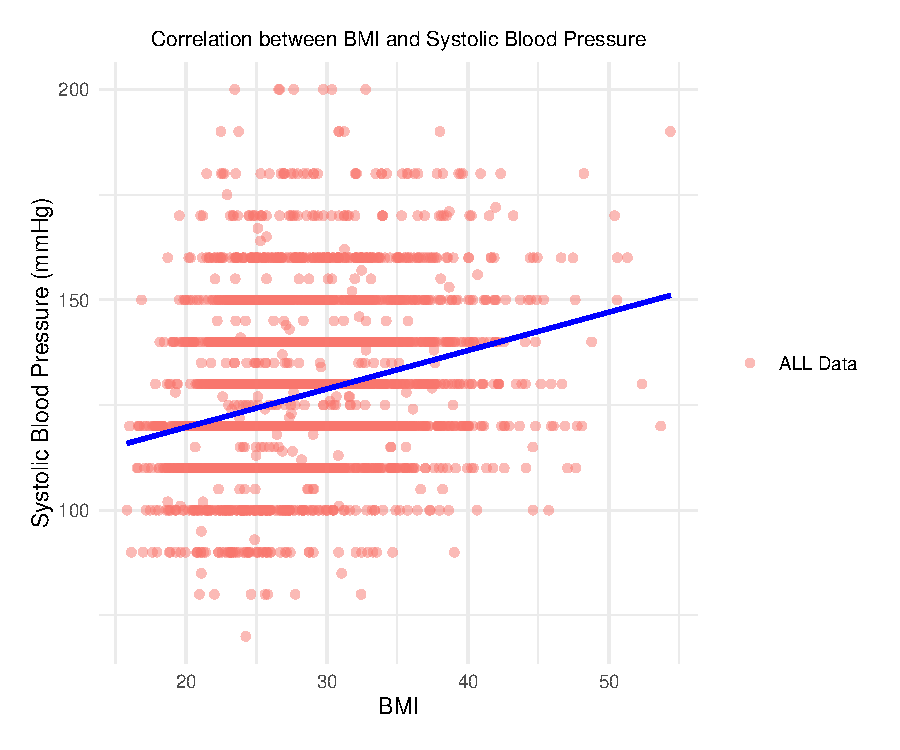
\includegraphics{home_work_test_files/figure-pdf/unnamed-chunk-8-1.pdf}
\end{center}

Answer: The Correlation coefficient between BMI and Systolic Blood
Pressure is 0.279. This correlation indicates a weak positive
correlation between BMI and systolic blood pressure. That means as BMI
increases, systolic blood pressure (ap\_hi) tends to increase slightly.
However, this relationship is not very strong.

To answer the question whether there is any difference between the two
classes of cardiovascular disease, we need to calculate the correlation
for the two classes separately and perform a Fisher's Z-test.

\begin{center}
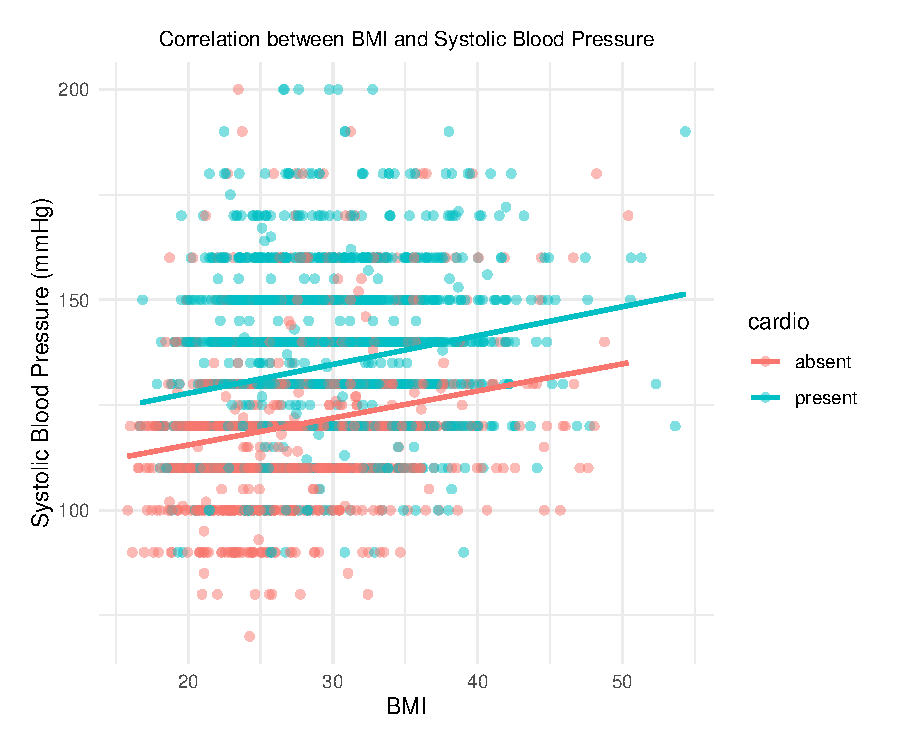
\includegraphics{home_work_test_files/figure-pdf/unnamed-chunk-9-1.pdf}
\end{center}

\begin{table}[!h]
\centering
\caption{Correlation between BMI and Systolic blood pressure grouped by cardio}
\centering
\begin{tabular}[t]{l|r}
\hline
\cellcolor[HTML]{D3D3D3}{\textbf{cardio}} & \cellcolor[HTML]{D3D3D3}{\textbf{Correlation}}\\
\hline
\cellcolor{gray!10}{absent} & \cellcolor{gray!10}{0.2317877}\\
\hline
present & 0.2136453\\
\hline
\end{tabular}
\end{table}

\begin{table}[!h]
\centering
\caption{Fisher's Z-test for Correlations between BMI and Systolic blood pressure grouped by cardio}
\centering
\begin{tabular}[t]{l|r}
\hline
\cellcolor[HTML]{D3D3D3}{\textbf{Metric}} & \cellcolor[HTML]{D3D3D3}{\textbf{Value}}\\
\hline
\cellcolor{gray!10}{Z\_score} & \cellcolor{gray!10}{0.666130}\\
\hline
P\_value & 0.505328\\
\hline
\end{tabular}
\end{table}

Based on the Fisher's Z-test, the Z score is 0.66613 and the P value is
0.505328. For the the Correlation coefficient between BMI and Systolic
Blood Pressure, there is no statistically significant difference between
the two groups of cardiovascular disease people based on the analyzed
metric. The observed results could be due to random variation rather
than a meaningful effect.




\end{document}
